\appendices
\onecolumn
% \begin{table}
% \begin{tabularx}{\textwidth}{|>{\raggedright\arraybackslash}X|>{\raggedright\arraybackslash}X|>{\raggedright\arraybackslash}X|>{\raggedright\arraybackslash}X|}
% \hline

% & \textbf{Fully Trusted Data Trust Assessment Function} 
% & \textbf{Fully Un-Trusted Data Trust Assessment Function} 
% & \textbf{Fully Dis-Trusted Data Trust Assessment Function} \\
% \hline

% \textbf{Operation on the first data of the test dataset} & 
% Belief: 0.856 \newline Disbelief: 0.042 \newline Uncertainty: 0.102 & 
% Belief: 0.287 \newline Disbelief: 0.05 \newline Uncertainty: 0.663 & 
% Belief: 0.0 \newline Disbelief: 1.0 \newline Uncertainty: 0 \\
% \hline

% \textbf{Feed Forward + Aggregation on Tx fully trust opinion} & 
% Belief: 0.846 \newline Disbelief: 0.053 \newline Uncertainty: 0.102 & 
% Belief: 0.298 \newline Disbelief: 0.043 \newline Uncertainty: 0.659 & 
% Belief: 0.0 \newline Disbelief: 1.0 \newline Uncertainty: 0 \\
% \hline

% \textbf{Feed Forward + Aggregation on Tx fully un-trust opinion} & 
% Belief: 0.839 \newline Disbelief: 0.053 \newline Uncertainty: 0.108 & 
% Belief: 0.296 \newline Disbelief: 0.043 \newline Uncertainty: 0.661 & 
% Belief: 0.0 \newline Disbelief: 1.0 \newline Uncertainty: 0 \\
% \hline

% \textbf{Feed Forward + Aggregation on Tx fully dis-trust opinion} & 
% Belief: 0.0 \newline Disbelief: 1.0 \newline Uncertainty: 0 & 
% Belief: 0.0 \newline Disbelief: 1.0 \newline Uncertainty: 0 & 
% Belief: 0.0 \newline Disbelief: 1.0 \newline Uncertainty: 0 \\
% \hline
% \end{tabularx}
% \caption{Comparison of PaTAS trust outputs under different Data Trust Assessment Functions}
% \label{tab:ptas_subjective_logic}
% \end{table}

\begin{table}[htbp]
\centering
% \renewcommand{\arraystretch}{1.5}
\scriptsize
\begin{tabularx}{\textwidth}{|p{3.5cm}|X|X|X|}
\hline
\textbf{PaTAS Components} & \textbf{Role} & \textbf{Functionality} & \textbf{How It Works} \\
\hline

\textbf{NN Interface (400)} & 
Serves as the primary link between the PaTAS and the neural network & 
Captures inputs during forward and deltas during backpropagation from NN & 
Allows real-time access to NN data, enabling Trust Node alignment and trust assessment \\
\hline
\textbf{Structure(graph) (101)} & 
Represents the mirrored architecture of the NN within PaTAS & 
Defines layout of Trust Nodes corresponding to each neuron (input, hidden, output) & 
Maintains synchronized processing between NN and PaTAS for trust evaluation \\
\hline
\textbf{Operators Mapping (103)} & 
Maps NN operations to trust-assessment counterparts in PaTAS & 
Defines how NN functions (e.g., activation, summation) become trust operations & 
Ensures PaTAS executes a matching trust operation when NN operates \\
\hline
\textbf{$\omega_\theta$ (Trust Function Parameters) (102)} & 
Defines parameters for Trust Functions applied at each node & 
Provides adjustable parameters (like weights) shaping Trust Functions & 
Can be adjusted based on feedback or initialization to fine-tune node-level trust \\
\hline
\textbf{$\mathcal{T}$ (Data Trust Assessment Function) (200)} & 
Assesses trust of any data (input or during operation) & 
Quantifies trust for data point, e.g., based on metadata & 
Used as attribute; result is passed to feedforward or parameter trust update process \\
\hline
\textbf{Feed Forward (325)} & 
Manages propagation of trust data from input to output nodes in PaTAS & 
Executes forward pass across Trust Nodes \newline Input: Trust scores \newline Output: Trust scores & 
Each Trust Node evaluates input, applies Trust Function, forwards result \\
\hline
\textbf{Parameter Trust Update (330)} & 
Adjusts trust values based on feedback or errors & 
Functions like backpropagation, but for trust instead of weights \newline Input: Trust scores, deltas & 
Modifies trust values over time to improve reliability of trust evaluations \\
\hline
\textbf{(Optional) Aggregation (440)} & 
Aggregates node-level trust into overall score & 
Uses summation, averaging, or custom aggregation \newline Input: Trust scores \newline Output: Trust Score & 
Combines trust data to produce holistic output trust score \\
\hline
\textbf{Gen CPTA (225)} & 
Retrieves relevant CPTA substructure for inference & 
Builds structure corresponding to active neurons \newline Input: activated neuron list \newline Output: trust score function & 
Performs trust assessment for currently involved neurons only \\

\hline
\end{tabularx}
\caption{PaTAS Components: Their Role, Functionality, and Operational Behavior}
\label{tab:ptas_table}
\end{table}


\section{Correspondence between SL operators, binary logic / set operators and SL notation}
% \begin{table}[h]
%     \centering
%     \begin{tabular}{l c | l}
%         \toprule
%         \textbf{SL operator (page)} & \textbf{Symbol} & \textbf{SL notation} \\
%         \midrule
%         Addition (p.95) & $+$ & $\omega_{x\cup y} = \omega_x + \omega_y$ \\
%         Subtraction (p.97) & $-$ & $\omega_{x\setminus y} = \omega_x - \omega_y$ \\
%         Complement (p.99) & $\neg$ & $\omega_x = \neg \omega_x$ \\
%         Multiplication (p.102) & $\cdot$ & $\omega_{x\cap y} = \omega_x \cdot \omega_y$ \\
%         Comultiplication (p.103) & $\sqcap$ & $\omega_{x\vee y} = \omega_x \sqcap \omega_y$ \\
%         Division (p.110) & $/$ & $\omega_{x \bar{\wedge} y} = \omega_x \sqcup \omega_y$ \\
%         Codivision (p.112) & $\sqcup$ & $\omega_{x \bar{\vee} y} = \omega_x \sqcup \omega_y$ \\
%         Multinomial product (p.118) & $\cdot$ & $\omega_{XY} = \omega_X \cdot \omega_Y$ \\
%         Deduction (p.133) & $\odot$ & $\omega_{y|X} = \omega_X \odot \omega_Y|X$ \\
%         Abduction (p.171) & $\sim$ & $\omega_{x|Y} = \omega_X \sim (\omega_Y|X, a_X)$ \\
%         Bayes' theorem (p.187) & $\approx$ & $\omega_{\tilde{x}|Y} = \tilde{\phi}(\omega_Y|X, a_X)$ \\
%         Joint opinions (p.199) & $\cdot$ & $\omega_{XY} = \omega_{Y|X} \cdot \omega_X$ \\
%         Constraint fusion (p.215) & $\oplus$ & $\omega_X^{A \& B} = \omega_X^A \oplus \omega_X^B$ \\
%         Cumulative Fusion (p.225) & $\bigoplus$ & $\omega_X^{A \diamond B} = \omega_X^A \bigoplus \omega_X^B$ \\
%         Averaging fusion (p.229) & $\odot$ & $\omega_X^{A \otimes B} = \omega_X^A \odot \omega_X^B$ \\
%         Weighted fusion (p.231) & $\oplus$ & $\omega_X^{A \circ B} = \omega_X^A \oplus \omega_X^B$ \\
%         CC-fusion (p.233) & \textcopyright & $\omega_X^{A \heartsuit B} = \omega_X^A \oplus \textcopyright \omega_X^B$ \\
%         Unfusion (p.238) & $\ominus$ & $\omega_X^{A \spadesuit B} = \omega_X^A \ominus \omega_X^B$ \\
%         Trust discounting (p.254) & $\otimes$ & $\omega_X^{[A:B]} = \omega_X^A \otimes \omega_X^B$ \\
%         \bottomrule
%     \end{tabular}
%     \caption{SL Operators and Corresponding Notations}
%     \label{tab:sl_operators}
% \end{table}
\begin{figure}
    \centering
    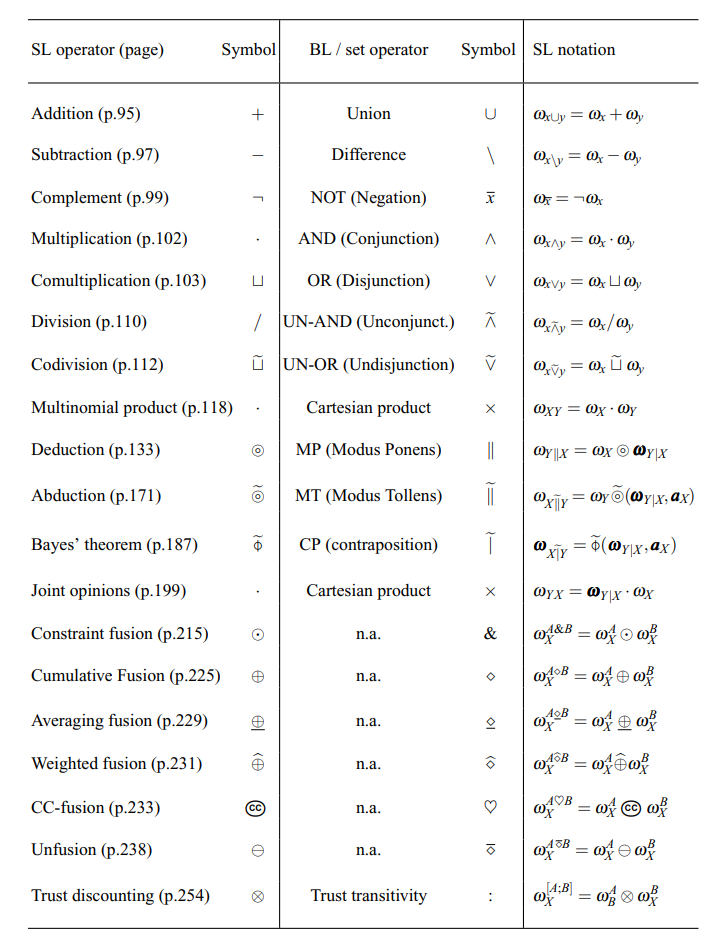
\includegraphics[width=0.5\linewidth]{img/opslist.png}
    \caption{Caption}
    \label{fig:enter-label}
\end{figure}
% you can choose not to have a title for an appendix
% if you want by leaving the argument blank
\section{Flow diagram and ...}

\begin{figure}
    \centering
    \includegraphics[width=0.5\linewidth]{slides/creation.png}
    \caption{Flow Diagram for Creation of a Parallel Trust Assessment System}
    \label{fig:creationdiagram}
\end{figure}


\begin{figure}
    \centering
    \includegraphics[width=0.8\linewidth]{slides/trustaggregation.png}
    \caption{Trust Aggregation}
    \label{fig:trustaggregation}
\end{figure}

\begin{figure}
    \centering
    \includegraphics[width=0.8\linewidth]{slides/IPTA.png}
    \caption{IPTA Generation}
    \label{fig:ipta}
\end{figure}


\section{}
Appendix two text goes here.


% use section* for acknowledgment
\section*{Acknowledgment}


The authors would like to thank...